% This is LLNCS.DEM the demonstration file of
% the LaTeX macro package from Springer-Verlag
% for Lecture Notes in Computer Science,
% version 2.4 for LaTeX2e as of 16. April 2010
%
\documentclass{llncs}
%
\usepackage[portuguese]{babel}
\usepackage[utf8]{inputenc}
\usepackage{makeidx}  % allows for indexgeneration

\usepackage{graphicx}
\usepackage{placeins}
\setcounter{secnumdepth}{3}
\graphicspath{ {./img/} }
%

\begin{document}

%
\frontmatter          % for the preliminaries
%
\pagestyle{headings}  % switches on printing of running heads
%
\title{Ano Escolar}
\subtitle{Resolução de Problemas de Desisão utilizando\\
Programação em Lógica com Restrições}
%
\titlerunning{Ano Escolar}  % abbreviated title (for running head)
%                                     also used for the TOC unless
%                                     \toctitle is used
%
\author{David Azevedo - up201405846 \and João Ferreira - up201404332}
%
\authorrunning{David Azevedo \and João Ferreira} % abbreviated author list (for running head)
%
\institute{Faculdade de Engenharia da Universidade do Porto\\
Rua Roberto Frias, sn, 4200-465 Porto, Portugal}

\maketitle              % typeset the title of the contribution

\begin{abstract} %

O objetivo deste trabalho é a criação de um programa, em Programação em Lógica com Restrições, capaz de marcar trabalhos de casa e testes para um periodo do ano, restritos a certas condições.

Ao longo deste documento será descrito o desenvolvimento do trabalho realizado, as metologias e abordagens diferentes assim como os resultados obtidos.

\end{abstract}
%
\section{Introdução}
%
Devido à complexidade combinatória existente no planeamento de um Ano Escolar, é necessária uma solução optima que permita obter da melhor forma um plano de aulas ágil e eficaz.

Este trabalho tem como objetivo, para um dado Ano Escolar, marcar os trabalhos de casa e os testes para diferentes turmas e disciplinas, dependendo de variáveis definidas pelo utilizador.
Neste documento está descrito detalhadamente o problema, uma abordagem de resolução do problema e uma análise sobre a mesma. Também será discutida a estratégia de pesquisa, os predicados de visualização e filamente uma conclusão geral sobre o trabalho.


\section{Descrição do Problema}
%
O problema de otimização escolhido foi o Ano Escolar, neste problema é proposto que, o programa desenvolvido , seja capaz de marcar trabalhos de casa e testes para um número indefinido de turmas e de semanas. Em relação aos trabalhos de casa, para cada turma existe um dia livre e o número de TPC só pode ser metade do número de ocorrências da disciplina não podendo existir mais que um número determinado de TPC's no mesmo dia. Em relação aos testes, cada disciplina tem dois testes, decorrendo num número de semanas especifico (meio e fim do período) e o número máximo de testes é dois por semana, sendo que não existem testes em dias consecutivos.

\section{Abordagem}
%
Num primeiro ato de abordagem ao problema, o problema foi dividido em dois subproblemas, a marcação dos trabalhos de casa e a marcação dos testes.

Para a marcação dos trabalhos de casa, foram realizados dois perdicados que resolvem o problema de dois pontos de vista diferente.

Para o primeiro predicado dos trabalhos de casa, foi utilizada uma estrutura de modo a limitar as variáveis utilizadas por disciplina, foi criada uma lista que contém os dias da semana, cada dia contem listas por disciplina com comprimento igual ao número de semanas para indicar, em que semanas existem ou não TPCs, naquela disciplina, daquele dia da semana. A razão pela qual foi optada esta  estrutura, foi numa tentativa de otimizar o espaço para representar os dias em que é possivél marcar trabalhos de casa para certa disciplina.
\newline

Para o segundo predicado dos trabalhos de casa, foi utilizada uma lista, onde cada index, indica a disciplina, e o elemento contido nesse index é um array de tamanho igual ao número de ocorrências dessa disciplina, ao longo do período de aulas. Esta estrutura permite ter em atenção a totalidade de ocorrências de uma dada disciplina, permitindo distribuir de melhor forma os trabalhos de casa.

No problema dos testes, optamos  por escolher uma estrutura que segue o seguinte formato : Uma lista de listas, onde cada lista representa uma turma, a lista da turma por sua vez tem uma lista para cada disciplina que por sua vez tem uma lista de dois elementos, a data do primeiro teste e a data do segundo (dia total, ou seja, semana * 5 + dia da semana). Achamos que esta seria uma boa estrutura uma vez que é organizada, direta e facilita a realização da maioria das restrições.

\subsection{Variáveis de Decisão}

Em relação aos trabalhos de casa, as variáveis de decisão são:

Para o primeiro predicado:
\begin{enumerate}
\item Dia Livre de Domínio [1,5], que representa um dos dias úteis da semana.
\item Lista de TPCs por disciplina de Domínio[0,1], que representa se existe ou não trabalho de casa em determinada semana, determinada pela sua posição.
\end{enumerate}

A lista de TPCs por disciplina, é um conceito simples, mas ligeiramente difícil de explicar, como foi descrito na secção anterior, cada disciplina de um determinado dia, tem associada uma lista, de tamanho igual ao número de semanas de aulas, em que cada posição da lista representa o número da semana e o seu conteúdo indica se existe ou não trabalho de casa, 1 em caso positivo 0 em caso negativo.

Para o segundo predicado:
\begin{enumerate}
\item Dia Livre de Domínio [1,5], que representa um dos dias úteis da semana.
\item Lista de Dias com TPC por disciplina de Domínio[0, DiasSemana ], que representa os dias em que existe trabalhos de casa, um valor maior que zero indica o dia do TPC.
\end{enumerate}

%
Em relação aos testes, existem 2 tipos de variaveis de dominios as variaveis para o primeiro teste e as variaveis para o segundo, no inicio da resolução do problema é calculado o intervalo para os primeiros testes e os segundos, que são representados como [Min1,Max1,Min2,Max2], estes valores representa (como dia total), o inicio e o fim de cada ronda de testes.

\begin{enumerate}
\item Dia Teste 1 de Domínio [Min1,Max1], que representa o primeiro intervalo dos testes.
\item Dia Teste 2 de Domínio [Min2,Max2], que representa o segundo intervalo de testes.
\end{enumerate}

\subsection{Restrições}

Na prespetiva dos trabalhos de casa, as restrições aplicadas são:

Para o primeiro predicado:
\begin{enumerate}
\item Para cada disciplina de um determinado dia, o número de trabalhos de casa tem que ser igual à metade do número de semanas de aulas.

Utilizando a estrutura descrita nas últimas secções, esta restrição faz-se simplesmente em prolog, utilizando o predicado count(1, Lista, \#=, Semanas/2) em que Lista representa, por disciplina de um determinado dia, as semanas em que existe TPC e Semanas o número total de semanas.

\item Para cada dia, o número de trabalhos de casa não pode superar uma variável definida pelo utilizador.

Para a implementação desta restrição, foram criados vários predicados com o intuito de, somar os nésimos elementos de um conjunto de listas, e verificar se esse valor é inferior ou igual ao número máximo de TPC's por dia.
\end{enumerate}

Para o segundo predicado:
\begin{enumerate}
\item Para cada lista de TPC's por disciplina, o número de ocorrências do número zero ( indicativo de que não existem trabalhos de casa) tem que ser igual à metade do número de ocorrêcias da disciplina, ao longo do ano (Esta razão pode ser presonalizada pelo utilizador).
Cada elemento desta lista é restrito para os dias em que ocorre a disciplina associada, como pode ser observado na seguinte condição:
\begin{equation}
\begin{array}{rcl}
 E &\subseteq& TPCList \\
 (E mod 5) &\subseteq& Ocurrs
\end{array}
\end{equation}

Onde ~$TPCList$ é a referida, lista de TPC's por disciplina, ~$E$ é um elemento dessa lista e ~$Ocurrs$ é uma lista que contém os dias da semana em que hà essa disciplina.

\item Para cada dia o número de trabalhos de casa não pode superar um máximo.
Esta restrição foi implementada numa prespetiva de tarefas, neste caso, cada tarefa tem duração e custo únitários e pretende-se descobrir os tempos iniciais de cada tarefa de modo a que nunca ultrapasse os recursos disponíveis : (limite máximo de tpc's).
\begin{equation}
\begin{array}{rcl}
 comulative( Tasks, [limit(N_{TPCs})])
\end{array}
\end{equation}
Para isso foi utilizado o predicado comulative, acima representado, que recebe um conjunto de tasks e como parâmetero options foi utilizado limit( número máximo de tpcs).

\end{enumerate}

Nos Testes, as restrições são:

\begin{enumerate}
\item Ter no máximo apenas dois testes por semana.

\item Não ter teste em dias consecutivos (nem sobrepostos).

\item Os testes realizados pelas diferentes turmas a uma mesma disciplina devem ser o mais próximos possível.

\item A Turma ter aula da disciplina no dia do teste.
\end{enumerate}

Para a primeira restrição, a solução elaborada consiste em converter os dias nas semanas correspondentes através do predicado mod/2, a restrição é feita sobre os valores dessa lista, indicando que nenhum valor pode ocorrer mais do que 2 vezes na lista com o uso do predicado nvalue/2, a lista das semanas é ordenada sem eliminar os duplicados e para cada conjunto de 3 valores consecutivos é aplicado o predicado por forma a garantir que existem pelo menos 2 valores diferentes nesses três elementos.

Para garantir que não haviam dois testes no mesmo dia foi utilizado o predicado all\_distinct/1. O predicado cumulative/2 foi utilizado para restringir os testes a não ficarem em dias consecutivos para isto foi criado um predicado que gerava as tasks e o principio básico foi que "cada teste começa no dia anterior é realizado no próprio dia e acaba no dia seguinte", ou seja, cada teste tem um custo de 3 dias sendo que o dia do meio é o dia em que este é realizado.

Para diminuir a distancia entre os testes de uma mesma disciplina para as diferentes turmas foram usadas duas estratégias, a primeira estratégia foi somar os dias dos testes para cada disciplina e minimizar essa forma, para isso definimos uma estrutura que é uma lista de listas onde cada lista elemento representa um teste de uma disciplina e cada um dos seus elementos representa o dia para as diferentes turmas, com esta estrutura feita e os valores somados, utilizamos a opção de minimize/2 no labeling por forma a encontrar a opção melhor. Devido ao elevado número de combinações quando temos muitas , turmas, disciplinas, semanas, etc. optámos por utilizar a nossa estrutura inicial já referida para minimizar as distância resolvendo as variavéis começando o mais a esquerda possível (leftmost), isto funciona uma vez que as disciplinas são resolvidas por onde para cada uma das turmas, sendo que a ordem é global, portanto a ordem de disciplina pela qual cada turma realiza um teste é sempre a mesma e é sempre encontrado o valor mais cedo possível para essa realização, sendo que a distância dos testes entre as turmas para a mesma disciplina são as menores que o solver como encontrar cumprindo as restriçoes. Por vezes esta solução não é a mais otimizada, mas sim uma das mais otimizadas, optámos por trocar este pequeno detalhe em prol de uma melhor performance para a procura em casos de dimensões superiores.

Por fim, apesar de não ser o caso na faculdade, no caso dos ensinos básico e secundário, os testes são realizados durante uma aula, o que implica que para o teste ser possível de ser realizado a turma deverá ter aula dessa disciplina nesse mesmo dia, portanto, apessar de não ser mencionado no enunciado o grupo decidiu implementar essa restrição. Esta restrição foi usada foi primeiro lugar uma vez que restringe imediatamente os dias que podem ser escolhidos. O principio aqui é : criar uma lista com uma lista para cada disciplina que contem os dias da semana em que a turma tem essa disciplina. Com esta lista restringimos os dominios dos dias dos testes para cada disciplinas convertendo cada lista no set usando o predicado list\_to\_fdset/2  e aplicando a restrinção ao dia - Dia in\_set DomainSet.


\subsection{Estratégia de Pesquisa}

Foi utilizada uma chamada ao labeling por defeito em todos os predicados de procura.


\section{Visualização da Solução}
Em relação aos trabalhos de casa:
Para o primeiro predicado:
O predicado que permite a visualização dos trabalhos de casa utiliza uma determinada turma, e os respetivos trabalhos de casa e representa da seguinte forma:
O nome do dia da semana, se o dia é livre ou não, seguido das disciplinas e cada disciplina indica as semanas em que existe TPC. Tal pode ser observado, com mais clareza na seguinte imagem:

\begin{figure}
\centering
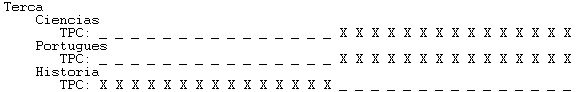
\includegraphics[width=1\textwidth]{tpc1}
\caption{Representação dos TPC's de uma disciplina}
\end{figure}
\FloatBarrier

%PICTURE!
Este predicado é iterado várias vezes dependendo do número de turmas existentes.

Para o segundo predicado:
É iterada a solução por disciplina e é imprimida a disciplina, o conjunto de semanas em que existe teste e o(s) respetivo(s) dia(s) da semana, tal pode ser observado na imagem seguinte:
%Picture!
\begin{figure}
\centering
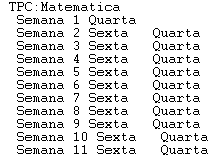
\includegraphics[width=0.4\textwidth]{tpc2}
\caption{Representação dos TPC's de uma disciplina}
\end{figure}
\FloatBarrier

Para os testes o resultado é mostrado por turma, para cada disciplina o dia do primeiro e segundo teste. Os números que representam os dias são números totais desde o inicio do periodo excluindo sábados e domingos. Por forma a ser de leitura simples e concisa. A divisão do valor por 5 devolve-nos a semana correspondente sendo que o mod nos devolve o  dia da semana.
Na imagem é possível observar o output da solução encontrada para 2 turmas com 5 disciplinas.
\begin{figure}
\centering
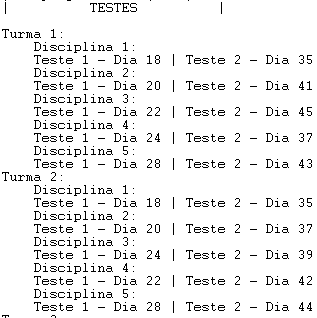
\includegraphics[width=0.7\textwidth]{testes}
\caption{Representação dos Testes para 2 Turmas com 5 Disciplinas}
\end{figure}
\FloatBarrier

\section{Resultados}

\subsection{ Trabalhos de Casa}

Para comparação dos dois perdicados, foram executados para a mesma turma, cada turma possiu 5 disciplinas distintas, um número variável de semanas, com limite de 2 trabalhos de casa por dia. Seguem-se a seguir os resultados.

\begin{figure}
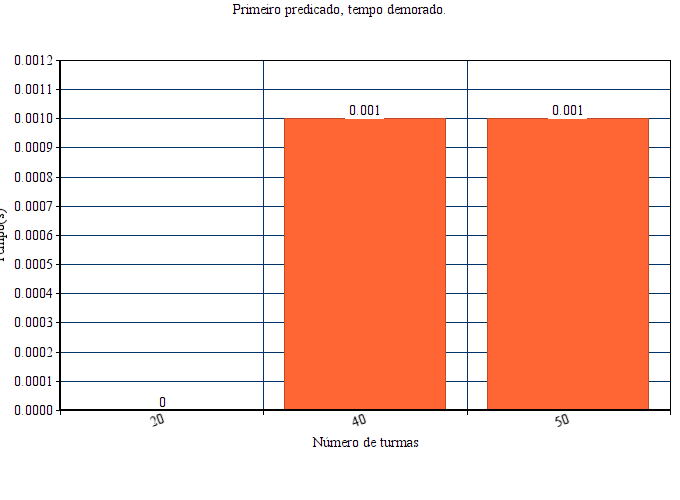
\includegraphics[width=0.5\textwidth]{g1}
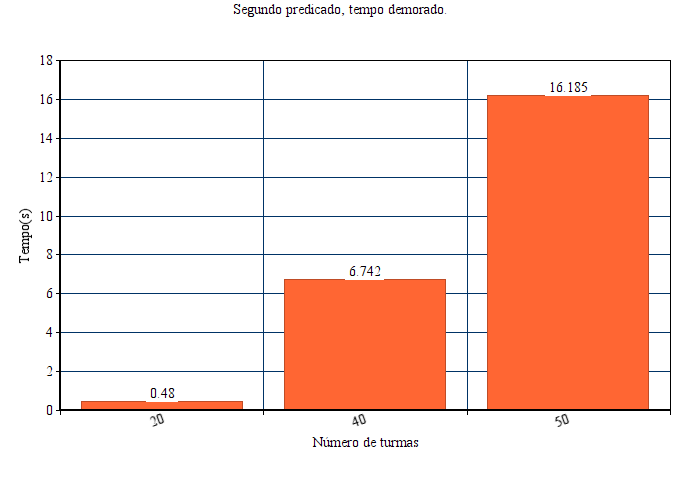
\includegraphics[width=0.5\textwidth]{g2}
\caption{Testes executados em ambos predicados}
\end{figure}
\FloatBarrier

Como é possível obervar o primeiro predicado teve um tempo de execução muito superior ao segundo, isto deve-se ao facto do uso de variáveis de domínio binárias e também por não se preócupar com o número de ocorrências da disciplina ao longo da semana, já que apenas marca TPC's para metade das semanas de aula de uma disciplina de um determinado dia.
Em relação ao segundo predicado, por ter estas condições em conta e pelas variáveis não estarem instânciadas de forma binária, quanto maior o número de semanas, relfete-se o aumento exponencial do tempo.

\subsection{ Testes}

Foram realizados 5 testes diferentes cada um deles com uma combinação diferente de complexidade, todos os resultados obtidos através dos métodos de estatisticas encontram-se nas imagens abaixo. Como é possível observar, o predicado que foi implementado é bastante rápido a encontrar uma solução, mesmo para problemas de grandes dimensões como é o caso da Figura \ref{reference}. Desde que hajam semanas suficientes para marcar os testes todos, e os horários se encontrem bem elaborados, isto é, as disciplinas que são dadas apenas 1 vez por semana não estejam todas no mesmo dia por exemplo, o predicado encontra uma solução ótima para o problema de uma forma muito ágil e eficaz. De notar ainda que a Figura \ref{refme} demorou um pouco mais uma vez que o espaço temporal era menor (10 semanas) em relação ao número de turmas e disciplinas.
\begin{figure}
\centering
    \begin{minipage}{0.45\textwidth}
    \centering
    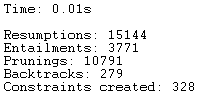
\includegraphics[width=.9\textwidth]{10Semanas_4Turmas_5Disciplinas}
    \caption{10 Semanas, 4 Turmas e 5 Disciplinas}
    \end{minipage}\hfill
    \begin{minipage}{0.45\textwidth}
    \centering
    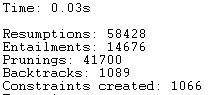
\includegraphics[width=0.9\textwidth]{10Semanas_13Turmas_5Disciplinas}
    \caption{10 Semanas, 13 Turmas e 5 Disciplinas}
    \label{refme}
    \end{minipage}\hfill
\end{figure}
\FloatBarrier

\begin{figure}
\centering
    \begin{minipage}{0.45\textwidth}
    \centering
    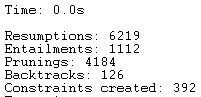
\includegraphics[width=.9\textwidth]{12Semanas_4Turmas_6Disciplinas}
    \caption{12 Semanas, 4 Turmas e 6 Disciplinas}
    \end{minipage}\hfill
    \begin{minipage}{0.45\textwidth}
    \centering
   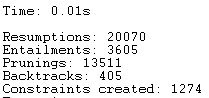
\includegraphics[width=.9\textwidth]{12Semanas_13Turmas_6Disciplinas}
\caption{12 Semanas, 13 Turmas e 6 Disciplinas}
    \end{minipage}\hfill
\end{figure}
\FloatBarrier

\begin{figure}
\centering
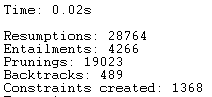
\includegraphics[width=0.45\textwidth]{25Semanas_12Turmas_7Disciplinas}
\caption{25 Semanas, 12 Turmas e 7 Disciplinas}
\label{reference}
\end{figure}
\FloatBarrier
\clearpage

\section{Conclusões}
Este projeto premitiu esclarecer vários conceitos relacionados com a programação em lógica com restrições, foi possivel, para o grupo, obter uma visão mais detalhada sobre este paradigma assim como a sua importância na resolução de diferentes problemas de otimização/decisão. Permitiu ainda uma melhor precepção sobre a importância da propagação das restrições de modo a melhorar o desempenho neste tipo de problemas.

Em relação aos trabalhos de casa:

Conclui-se que o primeiro predicado, devido à estrutura proposta para operar os dados foi possível otimizar a nivél de espaço o número de trabalhos de casa marcados, diminuindo consequentemente, o espaço de procura. A limitação trazida por esta estrutura é que, o plano escolar terá que ser tido em conta com semanas completas.  De modo a melhorar a especificação dos trabalhos de casa, poderão ser implementadas mais variáveis, de modo a fornecer mais flexibilidade no momento da pesquisa, como por exemplo, o dia livre ser variável de semana para semana, a utilização de listas de diferença de modo a melhorar o desempenho de como é feita a concatenação de listas, entre outros.

Conclui-se que o segundo predicado, devido à sua estrutura, foi capaz de minimizar o número de dias utilizados para marcar TPC's e foi possível a adaptação do predicado comulative, referênciado anteriormente. Em comparação com o primeiro predicado, utiliza uma estrutura muito mais flexivel, fácil de iterar, melhorias poderiam passar, por melhorar a procura do dia livre, esta procura é um fator importante no momento da pesquisa por soluções, um dia bem escolhido, já facilita bastante a marcação dos TPC's, a limitação realizada pelo grupo ainda é um bocado simplista, escolhendo os melhores dias para casos simples.

Em relação aos testes:

Além do que já foi referido nos parágrafos anteriores, podemos concluir que a forma como modulámos um problema e a estrutura que utilizámos para o representar representa um peso significativo no desempenho da solução encontrada pelo solver do sicstus. Uma vez que a estrutura nos facilitou a aplicação das restrições assim como reduzir imenso o dominio das variaveis, foi possível obter-se um predicado que nos resolve um problema do dia-a-dia numa pequenissima fração de segundo. Possui uma implementação muito fácil de compreender do ponto de vista lógico e muito flexivel no ponto de vista de acrescentar mais restrições. Um dos maiores desafios neste problema assim como no problemas dos trabalhos de casa foi a geração de uma estrutura de dados em prolog que visava a fácil intrepertação e manipulação das variaveis de dominio por forma a resolver os problemas da maneira mais rápida e eficiente possível.

O grupo sente-se orgulhoso com o resultado alcançado e capaz de afirmar, que se encontra familiarizado com o paradigma da programação em lógica com restrições para a resolução de problemas complexos e de otimização.

%
% ---- Bibliography ----
%
\pagebreak
\begin{thebibliography}{5}
%
\bibitem {url}
SWI-Prolog,
\url{http://www.swi-prolog.org}
\bibitem {url}
SICStus-Prolog,
\url{https://sicstus.sics.se}
\bibitem {url}
Effective Modeling with Constraints - Roman Barták,
\url{http://link.springer.com/chapter/10.1007\%2F11415763\_10}

\end{thebibliography}

\section*{Anexo}
\subsection*{Código fonte}

Bla Bla


\end{document}
